%%%%%%%%%%%%%%%%%%%%%%%%%%%%%%%%%%%%%%%%%
% a0poster Portrait Poster 
% LaTeX Template
% with University Copenhagen logo
% Version 1.0 (22/06/13)
%
% Based on:
% The a0poster class was created by:
% Gerlinde Kettl and Matthias Weiser (tex@kettl.de)
% 
% This template has been downloaded from:
% http://www.LaTeXTemplates.com
%
%%%%%%%%%%%%%%%%%%%%%%%%%%%%%%%%%%%%%%%%%

%----------------------------------------------------------------------------------------
%	PACKAGES AND OTHER DOCUMENT CONFIGURATIONS
%----------------------------------------------------------------------------------------

\documentclass[a1,portrait]{a0poster}
\usepackage[utf8]{inputenc}

\usepackage{multicol} % This is so we can have multiple columns of text side-by-side
\columnsep=70pt % This is the amount of white space between the columns in the poster
\columnseprule=3pt % This is the thickness of the black line between the columns in the poster

\usepackage[svgnames]{xcolor} % Specify colors by their 'svgnames', for a full list of all colors available see here: http://www.latextemplates.com/svgnames-colors

%\usepackage{times} % Use the times font
\usepackage{palatino} % Uncomment to use the Palatino font

\usepackage{graphicx} % Required for including images
\graphicspath{{figures/}{../img/}} % Location of the graphics files
\usepackage{booktabs} % Top and bottom rules for table
\usepackage[font=small,labelfont=bf]{caption} % Required for specifying captions to tables and figures
\usepackage{amsfonts, amsmath, amsthm, amssymb} % For math fonts, symbols and environments
\usepackage{wrapfig} % Allows wrapping text around tables and figures
\definecolor{tu}{RGB}{0,97,170}

\usepackage{framed}
\usepackage{tcolorbox}
\usepackage{lipsum}
\usepackage[compact]{titlesec}
\titlespacing{\section}{15pt}{*2}{*1}
\titlespacing{\subsection}{15pt}{*1}{*0}
\renewcommand\labelitemii{\textperiodcentered}
\setlength{\parindent}{15pt} % Default is 15pt.

\usepackage{tikz}
%\usetikzlibrary{babel}
\usetikzlibrary{positioning}
%\usetikzlibrary{shapes.geometric}
\usetikzlibrary{shapes,arrows}
\usetikzlibrary{backgrounds,fit}

\colorlet{shadecolor}{tu!20}

\usepackage[
backend=biber,
style=numeric,
citestyle=numeric-comp,
sorting=none,
natbib=true,
url=true, 
doi=false,
eprint=true
]{biblatex}
\addbibresource{sample.bib}

%Subfigures
\usepackage{subcaption}
\usepackage[export]{adjustbox}
\captionsetup{compatibility=false}
\usepackage[justification=centering]{caption}
\usepackage{wrapfig}

 \usepackage{eso-pic}
               \newcommand\BackgroundIm{
               \put(0,0){
               \parbox[b][\paperheight]{\paperwidth}{%
               \vfill
               \centering
               
\includegraphics[height=\paperheight,width=\paperwidth,
               keepaspectratio]{background.pdf}%
               \vfill
               }}}

\begin{document}
 \AddToShipoutPicture*{\BackgroundIm}
%----------------------------------------------------------------------------------------
%	POSTER HEADER 
%----------------------------------------------------------------------------------------

% The header is divided into two boxes:
% The first is 75% wide and houses the title, subtitle, names, university/organization and contact information
% The second is 25% wide and houses a logo for your university/organization or a photo of you
% The widths of these boxes can be easily edited to accommodate your content as you see fit



\begin{minipage}[t]{0.6\linewidth}
\vspace{4.7cm}
\Huge \color{Black} \textbf{Peppa Pig and Voronoi Diagrams}  \color{Black}\\ % Title
\huge Advanced Algorithmics project, fall 2017\\[0.5cm] % Subtitle
\Large \textbf{Mikhail Papkov}\\
\Large \textbf{Elizaveta Korotkova}\\[0.5cm] % Author(s)
\Large Institute of Computer Science\\ % University/organization

\end{minipage}
%
\begin{minipage}[t]{0.4\linewidth}
\color{DarkSlateGray}
\flushright
\vspace{5.1cm}
\Large \textbf{Repository:}\\
\texttt{git.io/vNmnd}\\[0.5cm]
\Large \textbf{Contacts:}\\
\texttt{mikhail.papkov@gmail.com}\\% Email address
\texttt{elizaveta.korotkova@gmail.com}% Email address
\end{minipage}

%\vspace{0.5cm} % A bit of extra whitespace between the header and poster content

%----------------------------------------------------------------------------------------
\def\columnseprulecolor{\color{tu}}
\begin{multicols}{2} % This is how many columns your poster will be broken into, a portrait poster is generally split into 2 columns

%----------------------------------------------------------------------------------------
%	ABSTRACT
%----------------------------------------------------------------------------------------

\color{tu} % Navy color for the abstract

\begin{abstract}
This poster presents the results of our participation in the project which was a part of the Advanced Algorithmics course at the Institute of Computer Science, University of Tartu. We have tried to approximate contour pictures with Voronoi diagrams using genetic optimization with different fitness functions.

\end{abstract}

%----------------------------------------------------------------------------------------
%	INTRODUCTION
%----------------------------------------------------------------------------------------

\color{Black} % SaddleBrown color for the introduction

\section*{Introduction}

\subsection*{Goals}
Our idea was to try to use Voronoi diagrams to approximate contour images and construct something similar to coloring pages.
A genetic algorithm was used for the approximation.

There exists a solution, in which a Voronoi diagram of several hundred points is used to
create a detailed polygon mesh of an image, using fuzzy k-means. We intended, however, to use relatively few points and to only approximate a contour of an uncolored image.  

\begin{center}
	\begin{minipage}{.4\linewidth}
		\centering
		
\includegraphics[width=.95\linewidth]{col/peppa.png}
		\captionof{subfigure}{Source image}
		\label{fig:source}
	\end{minipage}%
	~
	\begin{minipage}{.4\linewidth}
		\centering
		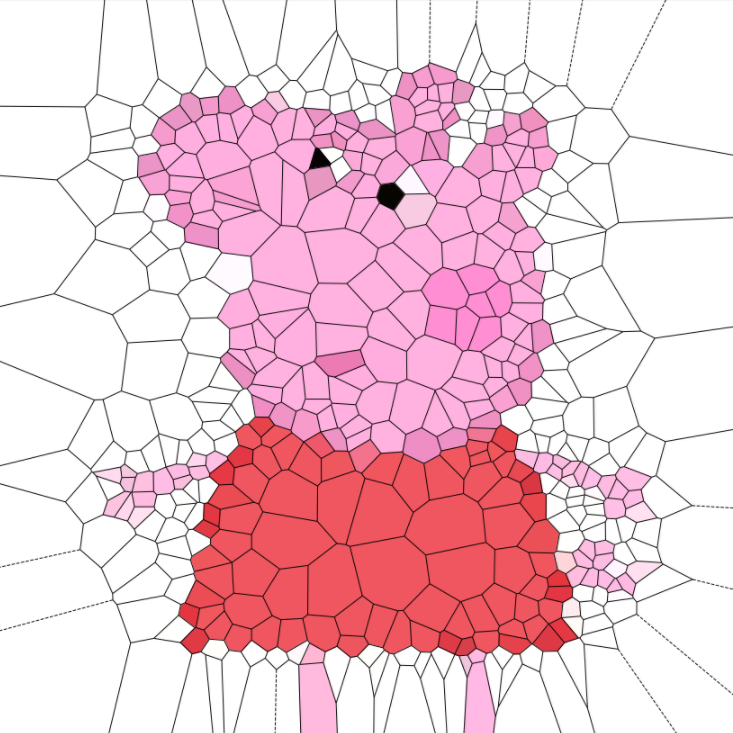
\includegraphics[width=.95\linewidth]{proc/peppa_500.png}
		\captionof{subfigure}{Processed image}
		\label{fig:fuzzy}
	\end{minipage}
	\captionof{figure}{Fuzzy k-means algorithm for contour detalization (500 centroids)}
\end{center}


\subsection*{Voronoi Diagrams}

A Voronoi diagram is a partitioning of a plane into regions based on a set of predefined points ${p_1 ... p_n}$ . The region of each point $p_i$ in this set
consists of every point in the Euclidean plane which is closer to $p_i$ than to any other point of the set.

We used \texttt{scipy.spatial.Voronoi} to generate diagrams from points.

\subsection*{Image Preprocessing}
The images were resized to $100\times100$ pixels for simpler shapes and to $150\times150$
for more complex ones. We used \texttt{skimage.morphology.skeletonize} to get thin,
1-pixel contours of the images.


%---------------------------------------

\section*{Genetic Algorithm}

%---------------------------------------
A genetic algorithm is a metaheuristic used in optimization and search problems, inspired by the process of natural selection. Its principle relies
on biological concepts like mutation, crossover and selection. Working process is the following:

%\begin{wrapfigure}{R}{0.4\linewidth}
%	\centering
%	
\includegraphics[width=0.9\linewidth]{proc/check.png} 
%	\caption{Algorithm demo for simple structure}
%	\label{fig:check}
%\end{wrapfigure}


\begin{itemize}
	\item Create an initial population of Voronoi diagrams (individuals).
	\item Choose the top diagrams (individuals) according to some cost function.
	\item Crossover: create a new diagram (individual) using points (genes) of the best diagrams
	selected at the previous step.
	\item Introduce random mutations to some points (genes) of the new individual,
	creating a new generation.
\end{itemize}

\subsection*{Parameters} 

\begin{itemize}
	\item Initialization (random; with centroids on the image skeleton)
	\item Number of centroids
	\item Population size
	\item Number of the best individuals chosen from each generation
	\item Mutation rate (how many centroids mutate)
	\item Mutation step (maximum by which the coordinates of a mutating centroid can change)
	\item Cost function (sum of distances vertex~--- skeleton; sum of top shortest distances vertex~--- skeleton; image overlap)
	\item Number of generations
\end{itemize}


\begin{center}
	
	\begin{minipage}{.5\linewidth}
		\centering
		
\includegraphics[width=.95\linewidth]{proc/check.png}
		\captionof{figure}{Algorithm demo for simple structure}
		\label{fig:skeleton1}
	\end{minipage}%
~
	\begin{minipage}{.5\linewidth}
		\centering
		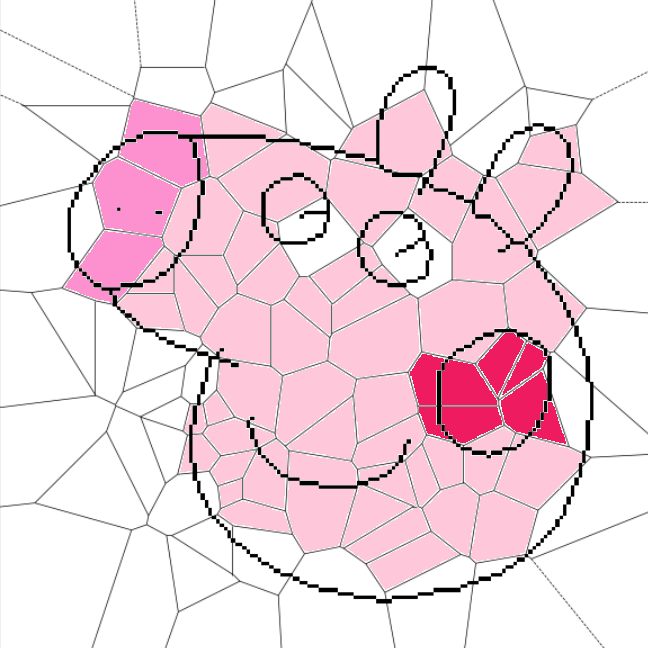
\includegraphics[width=.95\linewidth]{proc/randompeppa.png}
		\captionof{figure}{Initial diagram with random centroids}
	\end{minipage}
\end{center}




%----------------------------------------------------------------------------------------
%	RESULTS 
%----------------------------------------------------------------------------------------

\section*{Results}

\begin{center}
	\centering
	\begin{minipage}{.5\linewidth}
		\centering
		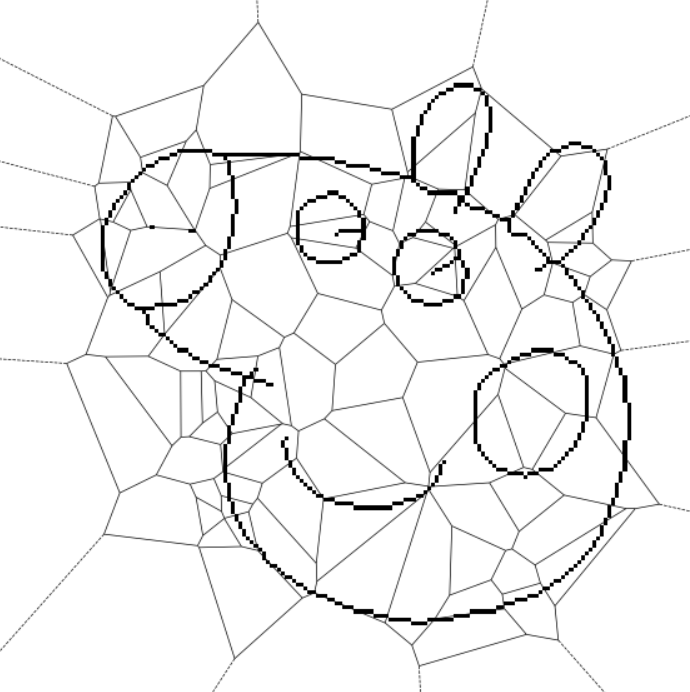
\includegraphics[width=.95\linewidth]{proc/peppa1_skeleton.png}
		\captionof{subfigure}{Skeletonized contour on the diagram}
		\label{fig:skeleton1}
	\end{minipage}%
	\begin{minipage}{.5\linewidth}
		\centering
		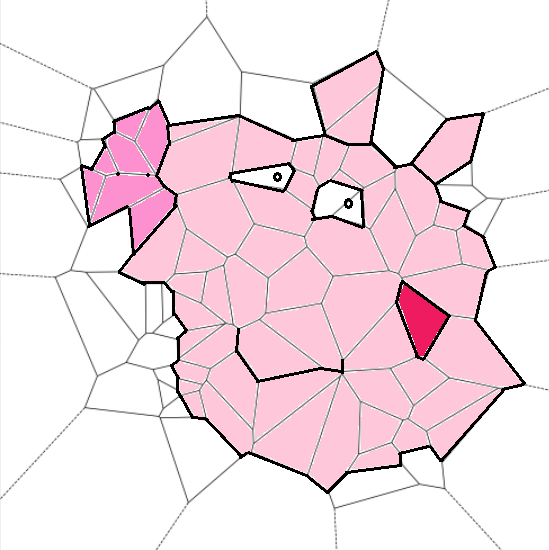
\includegraphics[width=.95\linewidth]{proc/peppa1_colored.png}
		\captionof{subfigure}{Colored diagram}
		\label{fig:colored1}
	\end{minipage}
	\captionof{figure}{Results of contour approximation (generations: 400, centroids: 100, population size: 30, mutation rate: 0.1, top selection: 5, max step: 3)}
\end{center}

We used different sets of parameters and different cost functions to generate the diagrams.
The algorithm does a more or less satisfactory job approximating simple shapes, while
more complex and more finely detailed images are harder.



 %----------------------------------------------------------------------------------------
%	REFERENCES
%----------------------------------------------------------------------------------------

%\nocite{*} % Print all references regardless of whether they were cited in the poster or not

%----------------------------------------------------------------------------------------
%	ACKNOWLEDGEMENTS
%----------------------------------------------------------------------------------------
\begin{wrapfigure}{r}{0.3\linewidth}
	
\includegraphics[width=.95\linewidth, right]{qr-code.pdf}
	\label{fig:qr}
\end{wrapfigure}

\section*{Acknowledgements}


We would like to thank Archimedes Foundation for the Dora Plus scholarships granted.

%
\includegraphics[width=.5\linewidth, right]{qr-code.pdf}



%----------------------------------------------------------------------------------------

\end{multicols}
\end{document}